\newpage
\hypertarget{multiEAP}{}
\subsection{Importing and working with multiple EAPs}
\genHeader

Please note that the following instructions on how to properly export and import Enterprise Architect (EA) files are \emph{not} an eMoflon-exclusive feature.
We have included them here as part of our handbook as getting this right is crucial for working with eMoflon, especially when working with TGGs. The main
problem is that, as far as we know, EA does not (yet) support referencing model elements in one EAP from another, completely different EAP. This means that all
required metamodels have to first be merged in the same EAP before such references can be specified (as required for TGGs).

\begin{itemize}

\item[$\blacktriangleright$] Press the \texttt{Install, configure and deploy Moflon} button and navigate to ``Install Workspace''.``Handbook Example (Part 4)''.
(Fig.~\ref{eclipse:dictionaryDownloadWizard}). Find and select ``Handbook Example (Part 4, 5)'' to copy a new \texttt{Dict\-ion\-ary\-Lang\-uage}
metamodel project into your workspace.
\newline
\vspace{0.5cm}

% Image stored in ../1_gettingStarted/visImportImages/
\begin{figure}[htbp]
\begin{center}
  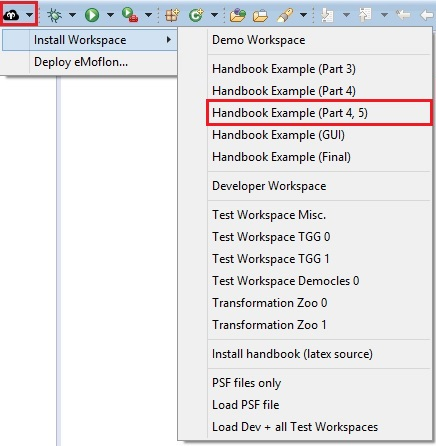
\includegraphics[width=0.8\textwidth]{eclipse_part4DictionaryLanguageDownload.jpg}
  \caption{Get the \texttt{DictionaryLanguage} metamodel}
  \label{eclipse:dictionaryDownloadWizard}
\end{center}
\end{figure}

\item[$\blacktriangleright$] If successful, your workspace should resemble Fig.~\ref{eclipse:loadedDictionaryEAP}. Double-click
\texttt{DictionaryVisual.eap} to open it in EA.

\begin{figure}[htbp]
\begin{center}
  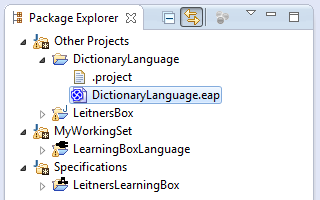
\includegraphics[width=0.5\textwidth]{eclipse_loadedDictionaryEAP}
  \caption{\texttt{Dictionary} metamodel successfully copied into the workspace}
  \label{eclipse:loadedDictionaryEAP}
\end{center}
\end{figure}

\item[$\blacktriangleright$] The file's project browser should resemble Fig.~\ref{ea:dictionaryLangStart}. Feel free to inspect the main
\texttt{DictionaryLanguage} diagram until you're familiar with the metamodel. Our work will be focused on the \texttt{Dictionary} and \texttt{Entry} classes.
You'll be able to see that dictionaries can be assigned unique \texttt{EString title}s, and each entry will have some sort of \texttt{content} matched with one
of three difficulty \texttt{level}s.

\vspace{0.5cm}

\begin{figure}[htbp]
\begin{center}
  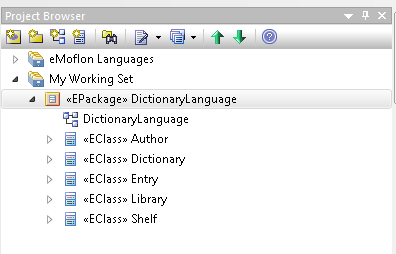
\includegraphics[width=0.4\textwidth]{ea_dictLangProBrowser}
  \caption{The \texttt{DictionaryLanguage} metamodel structure}
  \label{ea:dictionaryLangStart}
\end{center}
\end{figure}

\item[$\blacktriangleright$] It should be said that while you are able to simply copy and paste packages between multiple EAPs (i.e., copy
\texttt{<<E\-Pack\-age>>Dict\-ion\-ary\-Lang\-uage} into the \texttt{MyWorkingSet} root note \texttt{Leitners\-Learning\-Box\-Visual\-Spe\-ci\-fi\-ca\-tion.eap}), if any of the copied packages
have dependencies on other packages, it cannot be done so easily. All links would be destroyed! 

\clearpage

\item[$\blacktriangleright$] Therefore, to properly migrate the \texttt{DictionaryLanguage} package, right-click on the EPackage root, navigate to
``Import/Export" and select \texttt{Export Model to XMI\ldots} (Fig.~\ref{ea:contextExport}). Alternatively, you can select the root in the project browser and
press \texttt{Ctrl + Alt + E}.

%\vspace{0.5cm}

\begin{figure}[htbp]
\begin{center}
  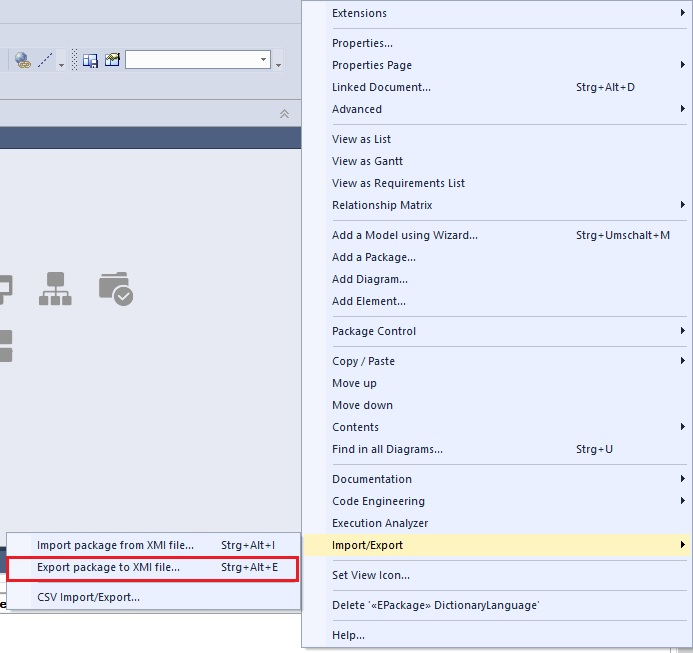
\includegraphics[width=\textwidth]{ea_contextExport}
  \caption{Starting the export process in EA}
  \label{ea:contextExport}
\end{center}
\end{figure}

\item[$\blacktriangleright$] Switch the export type to \texttt{XMI 2.1} in the dialogue and save the file somewhere easily accessible. Press export, and close
the window once the small blue bar appears (Fig.~\ref{ea:export}).

\begin{figure}[htbp]
\begin{center}
  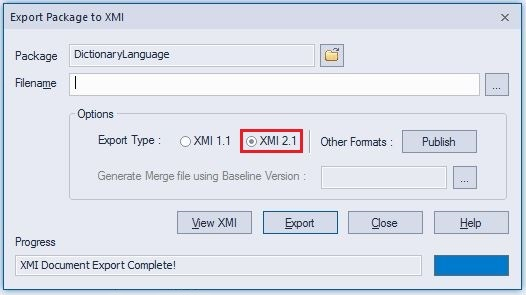
\includegraphics[width=0.9\textwidth]{ea_dialogueExport}
  \caption{Exporting the metamodel to a file}
  \label{ea:export}
\end{center}
\end{figure}

\item[$\blacktriangleright$] Go back to Eclipse and open \texttt{Leitners\-Learning\-Box\-Visual\-Spe\-ci\-fi\-ca\-tion.eap}. Right-click on \texttt{My Working Set} and navigate to ``Import
Model from XMI\ldots''

\item[$\blacktriangleright$] Find the \texttt{.xmi} file you just saved and
press \texttt{import}. Press \texttt{OK} in the confirmation dialogue. Your project browser should now resemble Fig.~\ref{ea:importProBrowser}, with both metamodels in the same working set, in the same EAP.

\begin{figure}[htbp]
\begin{center}
  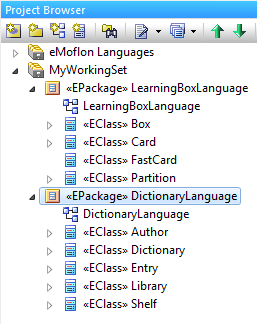
\includegraphics[width=0.5\textwidth]{ea_loadedDictionaryMetamodel}
  \caption{The TGG metamodels successfully included in one EAP}
  \label{ea:importProBrowser}
\end{center}
\end{figure}

\clearpage

\item[$\blacktriangleright$] Confirm the import by validating\footnote{To review the details of how to use the eMoflon control panel, read Section 2.8 from
Part II} (Fig.~\ref{ea:importValidationWindow}) and exporting the dual-metamodel project to Eclipse, refreshing \texttt{Leitners\-Learning\-Box\-Vi\-su\-al\-Spe\-ci\-fi\-ca\-tion} to rebuild your workspace. 

\vspace{0.5cm}

\begin{figure}[htbp]
\begin{center}
  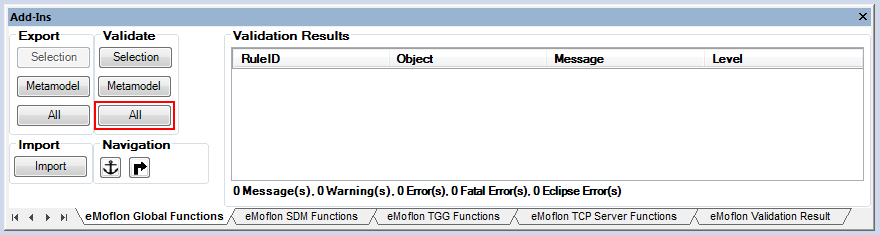
\includegraphics[width=\textwidth]{ea_importValidationWindow}
  \caption{No validation errors for \texttt{Leitners\-Learning\-Box\-Visual\-Spe\-ci\-fi\-ca\-tion}}
  \label{ea:importValidationWindow}
\end{center}
\end{figure}

\vspace{0.5cm}

\item[$\blacktriangleright$] That's it! You now have the second metamodel for your transformation prepared, and are ready to start specifying your TGG rules.

\end{itemize}
